%! TEX root = ../thesis.tex
\section{Experimental Results}
\label{clm:sec:results}

Starting with no information at all, we arbitrarily set the prior noise $\sigma_n^{2} = 1$ and the prior covariance matrix to a spherical covariance $\vec{\Sigma}_p = \sigma_p^{2} \vec{I}$, with $\sigma_p^{2} = 10$.
Our results are qualitatively robust to a large range of values for $\sigma_p^{2}$.
In order to compare the perceived carbon footprint $\exp \overline{\vec{w}}$ with its true value $\exp \vec{v}$, we set the prior mean to $\vec{\mu} = c \vec{1}$, where $ c = \frac{1}{M}\sum_{i=1}^M v_i$ is the mean of the (log-)true values.
This guarantees that the perceived carbon footprint estimated from the model parameters have the same scale as the true values.

We compile a set $\mathcal{A}$ of $M=18$ individual actions about transportation, food, and household (the full list of actions is provided in Appendix~\ref{app:clm:actions}).
We deploy an online quiz\footnote{Accessible at \url{http://www.climpact.ch}} to collect pairwise comparisons of actions from real users on a university campus (see Appendix~\ref{app:clm:climpact})
We collect $N=2183$ triplets from 176 users, mostly students between 16 and 25 years old.
We show in Figure~\ref{clm:fig:perception} the true carbon footprint, together with the global perception of the population, \textit{i.e.}, the values $\exp \overline{w}_i$ for each action $i \in \mathcal{A}$.

\begin{figure}
	\centering
	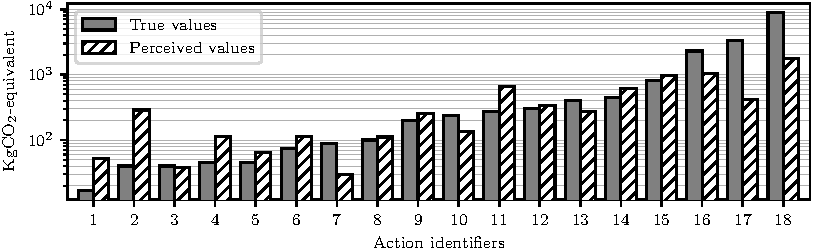
\includegraphics{clm-perception}
	\caption{Global perceived carbon footprint of 18 actions in kg\COtwo-equivalent and their true values (log scale).
		The list of actions is provided in Appendix~\ref{app:clm:actions}.}%
	\label{clm:fig:perception}
\end{figure}

The users in our population have a globally accurate perception.
Among the actions showing the most discrepancy, the carbon footprint of short-haul flights is \textit{overestimated}~(Action 11), whereas the carbon footprint of long-haul flights~(16) is highly \textit{underestimated}~(the scale is logarithmic).
Similarly, the carbon footprint of first-class flights~(18) is also \textit{underestimated}.
The users tend to \textit{overestimate} the carbon footprint of more ecological transports, such as the train, the bus, and car-sharing~(1, 4, and 6).
The users have an accurate perception of actions related to diet~(8, 14, and 15) and of actions related to domestic lighting~(3 and 10).
They \textit{overestimate}, however, the carbon footprint of a dryer~(2).
Finally, they highly \textit{underestimate} the carbon footprint of oil heating~(17).
Switzerland, where the users live, is one of the European countries whose consumption of oil for heating houses is the highest.
There is, therefore, a high potential for raising awareness around this issue.
